\documentclass[12pt]{report}
\usepackage[utf8]{inputenc}
\usepackage{graphicx}
\usepackage{ragged2e}
\usepackage{listings}
\usepackage{hyperref}
\usepackage[italian]{babel}     %usare questo per rendere tutto in                                    Italiano


\graphicspath{{images/}}


\hypersetup{
    colorlinks=true,
    linkcolor=blue,
    pdftitle={Relazione progetto Internet Security}
}


\title{
    {
\includegraphics[scale=0.4]{UniCT-Logo.jpg}}\\
    {Breve analisi di Maltego e della vulnerabilità CVE-2020-24656}\\
    {\large Università degli Studi di Catania}
}


\author{Mattia Maria Scivoletto}
\date{\today}

\renewcommand*\contentsname{Sommario}

\begin{document}
\maketitle


\tableofcontents

\chapter{Breve introduzione a Maltego e OSINT}
\begin{flushleft}
Con il termine \textbf{OSINT} (Open Source Intelligence), si intende l'attività di raccolta di informazioni pubblicamente disponibili e quindi libere (da qui il significato di open source) con l'intento di perseguire un certo obiettivo. L'OSINT è diventata un'attività fondamentale, soprattutto grazie all'enorme quantità di dati che viene prodotta, dati che rappresentano una fonte di ricchezza sia in ambito business che non. Bisogna prendere coscienza di questo genere di attività, dal momento che molti attacchi sono frutto dello sfruttamento di falle di cui si può venire a conoscenza semplicemente applicando delle tecniche di open source intelligence. Ecco perchè è importante capire se un'organizzazione espone delle informazioni sensibili che potrebbero di fatto renderla debole. Le fonti da cui si traggono le informazioni sono le più svariate: media come TV, giornali, radio, riviste, ma anche social media, blog, siti web, pubblicazione accademiche, basi di dati, report governativi, record whois, record DNS. Le informazioni che è possibile raccogliere sono di tanti tipi: indirizzi IP, indirizzi URL, email, informazioni su persone fisiche. L'OSINT è un'attività che viene svolta da molti soggetti differenti, e l'obiettivo ultimo dell'OSINT cambia di conseguenza. I principali soggetti che praticano OSINT sono:


\begin{itemize}
    \item i \textbf{penetration tester}, che vogliono scoprire quali informazioni sono pubblicamente disponibili e che un'attaccante potrebbe sfruttare a proprio vantaggio per studiare la vittima e condurre un'attacco
    \item le \textbf{forze dell'ordine}, che devono perseguire reati informatici come il cyberbullismo, e a cui interessa conoscere il criminale che sta perpetrando il reato per poterlo poi perseguire penalmente
    \item le \textbf{agenzie di intelligence statali}, che svolgono attività di spionaggio dentro e fuori i confini nazionali
    \item i \textbf{black hat}, che prima di attaccare la vittima la studiano, facendo attività di information gathering, detta anche reconaissance, allo scopo di scoprire i punti deboli del target. Chiaramente, più informazioni un'attaccante trova, migliore è l'idea che l'attaccante si fa della vittima 
\end{itemize}


Passando alle tecniche di open source intelligence, è bene sottolineare che è sconsigliato raccogliere qualsiasi informazione sul proprio target, dato che il volume di informazioni che ci troveremmo a gestire sarebbe troppo elevato e questo risulterebbe controproducente. Bisogna capire invece lo specifico aspetto che ci interessa approfondire della vittima, e raccogliere informazioni solo su quello. Inoltre è bene fare uso di tool e programmi che permettano di automatizzare la raccolta delle informazioni, in modo da essere più veloci ed efficaci nel raccogliere e catalogare i dati. Parlando degli strumenti per fare OSINT, quello che verrà trattato in questa sede è \textbf{Maltego}, prodotto dalla software house sudafricana Paterva, che permette di fare OSINT in maniera automatizzata, e consente di creare dei grafici basati su nodi, come dei grafi, in modo da avere una rappresentazione grafica dei dati raccolti. Maltego offre la possibilità di connettere facilmente dati e funzionalità da diverse fonti utilizzando Transforms. Tramite il Transform Hub, si possono collegare i dati di oltre 30 partner di dati, una varietà di fonti pubbliche (OSINT) e i propri dati. Esistono tante versioni di Maltego, più o meno gratuite e con una diversa ricchezza di funzionalità. La versione che verrà utilizzata è la Community Edition.
\end{flushleft}

\chapter{Breve introduzione alla vulnerabilità CVE-2020-24656}
\begin{flushleft}
La vulnerabilità \textbf{CVE-2020-24656} riguarda un attacco \textbf{XXE} (XML External Entity) che è possibile condurre ai danni di Maltego. XML External Entity è una vulnerabilità che consente a un utente malintenzionato di interferire con l'elaborazione di dati XML da parte di un'applicazione. Spesso consente a un utente malintenzionato di visualizzare i file sul filesystem del server delle applicazioni e di interagire con qualsiasi sistema di back-end o esterno a cui l'applicazione stessa può accedere. Alcune applicazioni utilizzano il formato XML per trasmettere i dati tra il browser e il web server. Le applicazioni che eseguono questa operazione utilizzano praticamente sempre una libreria standard o un'API della piattaforma per elaborare i dati XML sul server. Le vulnerabilità XXE sorgono perché il linguaggio XML contiene varie funzionalità potenzialmente pericolose e i parser standard supportano queste funzionalità anche se non sono normalmente utilizzate dall'applicazione. Questa vulnerabilità riguarda le versioni 4.2.11 e precedenti di Maltego. L'attacco permette di elaborare i file MTZ (contenenti le informazioni di configurazione) e MTGL (contenenti le informazioni sul grafo), in maniera tale da ottenere certe conseguenze, come ad esempio information disclosure, esecuzione di codice attraverso SSRF e denial of service. I file MTGL e MTZ sono dei file proprietari di Maltego, molto simili ai file ZIP (anch'essi sono in formato compresso). In questo particolare attacco, la vulnerabilità permette ad un attaccante di esfiltrare i file locali dal computer della vittima. A causa del fatto che i file MTGL e MTZ sono abbastanza spesso condivisi tra collaboratori e terze parti, le possibilità che qualcuno cada vittima di questa vulnerabilità sono relativamente alte.
\end{flushleft}

\chapter{Sistema operativo e versione di Maltego utilizzata}
La versione di Kali Linux utilizzata è la 2020.2, mentre la versione di Maltego utilizzata per condurre l'esperimento è la 4.2.3. La scelta di questa versione è motivata dal fatto che l'attacco ha effetto solo su Maltego 4.2.11 e versioni precedenti.

\chapter{Esperimento condotto}
\begin{flushleft}
Per comprendere appieno il pericolo delle entità esterne, è importante prima capire che cos'è un'entità. Le entità sono variabili XML a cui è possibile fare riferimento dall'applicazione. Gli sviluppatori utilizzano le entità per definire i valori e utilizzano tali valori nel codice futuro.
\end{flushleft}

\begin{flushleft}
Esempio di entità:
\end{flushleft}

\begin{lstlisting}[language=XML]
<?xml version="1.0"?>
<!DOCTYPE example [
    <!ENTITY hello "Hello world!">
]>
<User>
    <Name>Admin</Name>
    <DisplayName>Administrator</DisplayName>
    <Message>&hello;</Message>
</User>
\end{lstlisting}

\begin{flushleft}
In questo esempio, il contenuto del tag "Message" verrà popolato dall'entità "hello" appena definita.
\end{flushleft}

\begin{flushleft}
Allora cosa sono le \textbf{entità esterne}?
\end{flushleft}

\begin{flushleft}
Sono fondamentalmente la stessa cosa, tuttavia consentono di definire entità con dati esterni, mentre con le entità normali occorre definire esplicitamente i dati che vengono archiviati.
\end{flushleft}

\begin{flushleft}
Per creare un'entità esterna, occorre utilizzare la parola chiave "SYSTEM", seguita da un URL, che indicherà all'applicazione di recuperare il contenuto da quella risorsa esterna.
\end{flushleft}

\begin{flushleft}
Esempio di entità esterna:
\end{flushleft}

\begin{lstlisting}[language=XML]
<?xml version="1.0"?>
<!DOCTYPE example [
    <!ENTITY hello SYSTEM "https://www.google.com/robots.txt">
]>
<User>
    <Name>Admin</Name>
    <DisplayName>Administrator</DisplayName>
    <Message>&hello;</Message>
</User>
\end{lstlisting}

\begin{flushleft}
Questo frammento recupererà i contenuti dall'URL fornito e li memorizzerà nell'entità "hello". La cosa interessante delle entità esterne è che non si è limitati alle risorse "esterne".
\end{flushleft}

\begin{flushleft}
Utilizzando diversi protocolli URI, possiamo interagire con altre risorse. Se vogliamo leggere un file locale del server o del PC della vittima, possiamo usare il seguente URI.
\end{flushleft}

\begin{flushleft}
file:///etc/passwd
\end{flushleft}

\begin{flushleft}
Ora che abbiamo ottenuto il contenuto del file archiviato in una variabile, possiamo creare un'altra entità esterna per inviare una richiesta al nostro server malevolo con i contenuti. Una volta inviata la richiesta al nostro server, possiamo controllare i log di accesso e osservare il contenuto del file.
\end{flushleft}

\begin{flushleft}
\textbf{Panoramica sull'exploit}
\end{flushleft}


\begin{flushleft}
Affinché un utente malintenzionato possa sfruttare con successo questa vulnerabilità, dovrebbe convincere una vittima ad aprire un file MTZ o MTGL all'interno di Maltego. Questo è abbastanza comune poiché Maltego utilizza questi file per memorizzare il grafo e le varie impostazioni di progetto.
\end{flushleft}

\begin{flushleft}
Ad esempio, i file MTGL/MTGX sono essenzialmente file di progetto.
\end{flushleft}

\begin{flushleft}
I file MTZ, tuttavia, sono usati esclusivamente per le configurazioni, come nuove transform, nuove entità, ecc.
\end{flushleft}

\begin{flushleft}
\textbf{Panoramica tecnica}
\end{flushleft}

\begin{flushleft}
Per questo esempio useremo un file di grafo perché questi sono i meno sospettabili e sono spesso condivisi tra altre persone. Il primo passaggio consiste nel creare un file di grafo vuoto e trascinare un'entità nella vista. Fatto ciò, possiamo salvarlo e iniziare a modificare le cose all'interno del file MTGL.
\end{flushleft}

\begin{flushleft}
La prima cosa che si nota riguardo i file MTGL/MTZ è che in realtà sono semplicemente un insieme di file XML e di file di proprietà, compressi in un archivio ZIP. Questo rende molto semplice il "reverse engineering" dei formati di file di Maltego.
\end{flushleft}

\begin{flushleft}
Ecco uno screenshot che mostra il file MTGL su cui faremo l'esperimento:

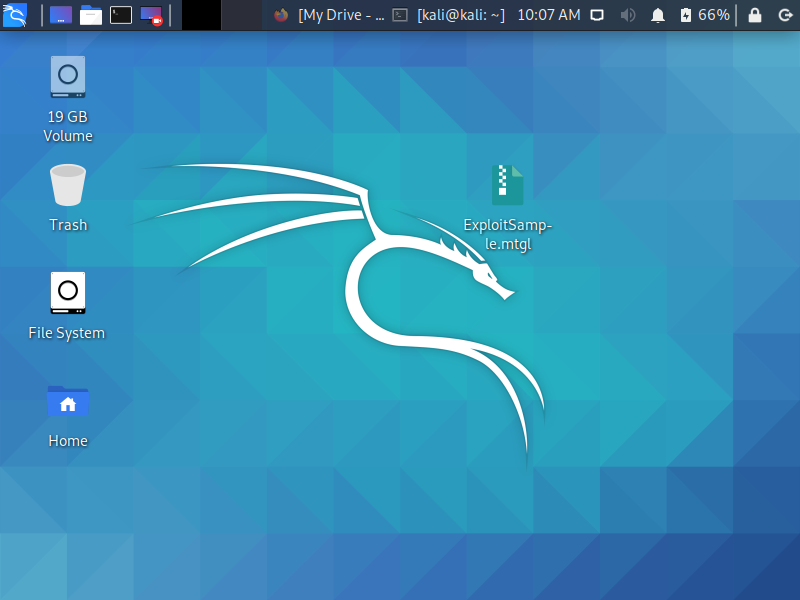
\includegraphics[scale=0.5]{images/Screenshot-file-MTGL-Maltego.png}
\end{flushleft}

\begin{flushleft}
Ecco quello che accade se decomprimiamo il file ExploitSample.mtgl:

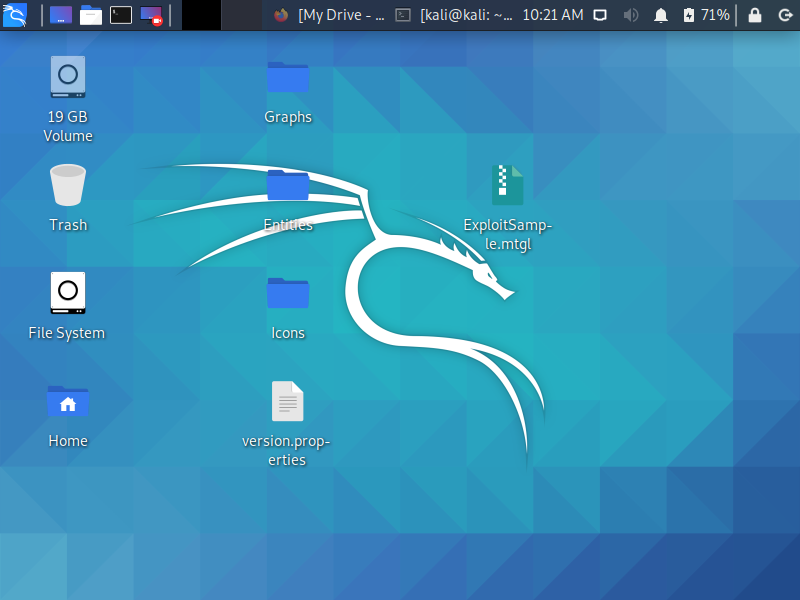
\includegraphics[scale=0.5]{images/Screenshot cartelle interne file MTGL.png}
\end{flushleft}

\begin{flushleft}
Il file MTGL contiene dunque 3 cartelle, Graphs, Entities e Icons, ed un file denominato version.properties.
\end{flushleft}

\begin{flushleft}
L'idea qui è di modificare uno dei file XML e aggiungere il nostro payload, per poi reimpacchetare il file MTGL per inviarlo alla vittima.
\end{flushleft}

\begin{flushleft}
In questo esempio modificheremo una delle entità, che di default è simile alla seguente:
\end{flushleft}

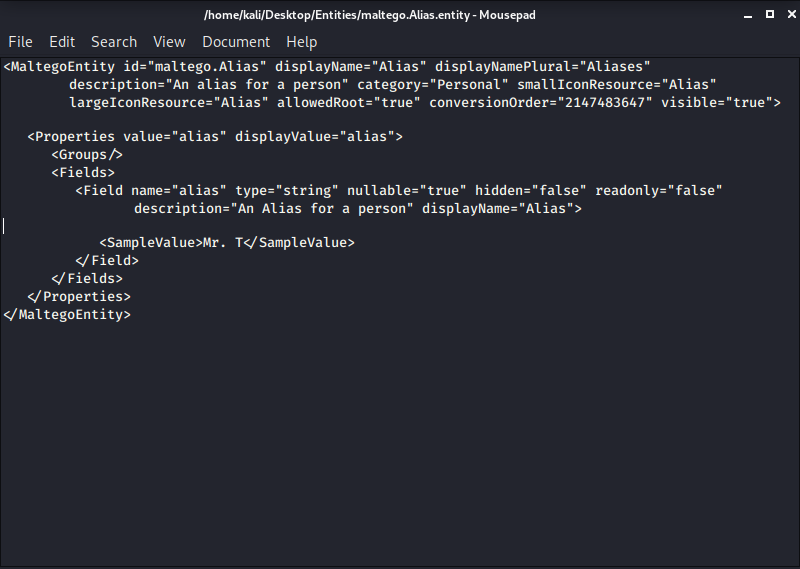
\includegraphics[scale=0.5]{images/Screenshot-file-maltego.Alias.entity.png}

\begin{flushleft}
Tutto ciò che dobbiamo fare è aggiungere un'entità, quindi fare in modo che faccia riferimento a un altra entità esterna che sarà responsabile dell'esfiltrazione.
\end{flushleft}

\begin{flushleft}
Ecco il file con l'aggiunta del payload:
\end{flushleft}

\includegraphics[scale=0.5]{images/Screenshot file entità con payload.png}

\begin{flushleft}
Ed ecco il contenuto del file lol.dtd:
\end{flushleft}

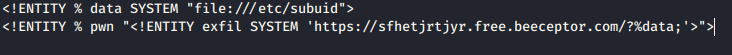
\includegraphics[scale=0.5]{images/Screenshot file lol.dtd.png}

\begin{flushleft}
Per ragioni di test, verrà usato beeceptor.com, che è principalmente usato per REST API mocking. Beeceptor ci consente di settare delle regole mock API, permettendoci di hostare lì il contenuto del file letto dalla macchina vittima.
\end{flushleft}

\begin{flushleft}
Ad alto livello, ecco come funziona il payload. Innanzitutto, creiamo un'entità che acquisisca il contenuto del file lol.dtd dall'URL fornito.
\end{flushleft}

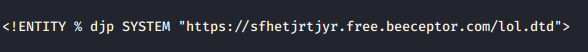
\includegraphics[scale=0.6]{images/Screenshot_1.png}

\begin{flushleft}
Quindi, nel file lol.dtd, creiamo un'altra entità che acquisisca il contenuto del file locale scelto.
\end{flushleft}

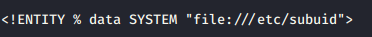
\includegraphics[scale=0.5]{images/Screenshot_2.png}

\begin{flushleft}
Infine, definiamo un'altra entità, che invierà una richiesta GET con i contenuti dell'entità "data" che abbiamo creato. Essenzialmente stiamo esfiltrando il contenuto del file.
\end{flushleft}

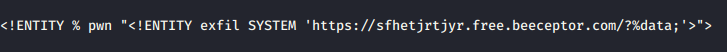
\includegraphics[scale=0.5]{images/Screenshot_3.png}

\begin{flushleft}
Ora, quando Maltego tenta di eseguire il rendering dell'entità, il tag SampleValue avrà come valore quello dell'entità esterna "exfil":
\end{flushleft}

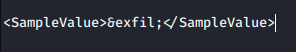
\includegraphics[scale=0.7]{images/Screenshot_4.png}

\begin{flushleft}
Il parser XML leggerà la definizione della nostra entità "exfil", valutando in definitiva le nostre entità istantaneamente quando viene eseguito il rendering del file grafico.
\end{flushleft}

\begin{flushleft}
Ora che abbiamo compreso come funziona l'attacco, possiamo andare avanti e testarlo. Creiamo un semplice file di grafo come è stato fatto vedere precedentemente. Una volta che abbiamo fatto, possiamo decomprimere il file col seguente comando:
\end{flushleft}

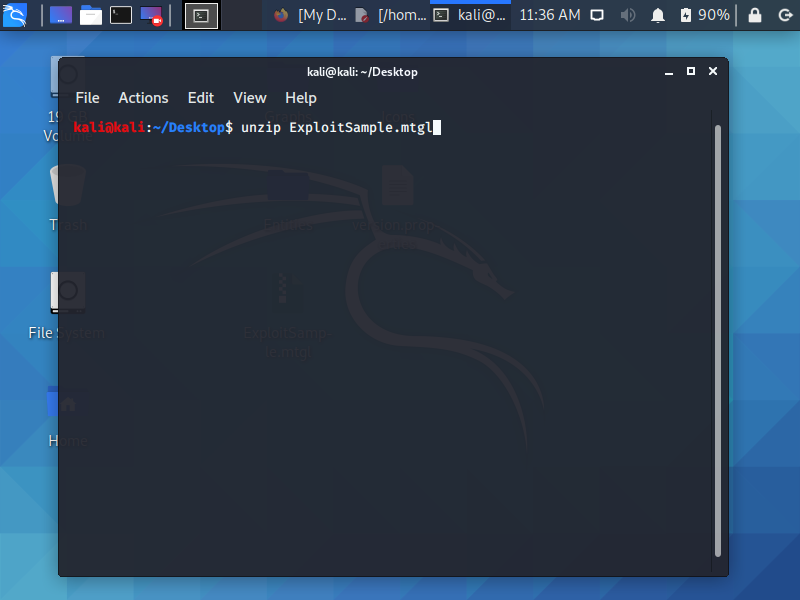
\includegraphics[scale=0.4]{images/Screenshot unzip file MTGL.png}

\begin{flushleft}
Ora possiamo modificare il file "Entities/maltego.Alias.entity", con i seguenti contenuti:
\end{flushleft}

\includegraphics[scale=0.4]{images/Screenshot file entità con payload.png}

\begin{flushleft}
Dobbiamo anche impostare la regola su beeceptor, affinché alla ricezione di una richiesta HTTP di tipo GET del file lol.dtd, il nostro server restituisca in risposta il contenuto del file.
\end{flushleft}

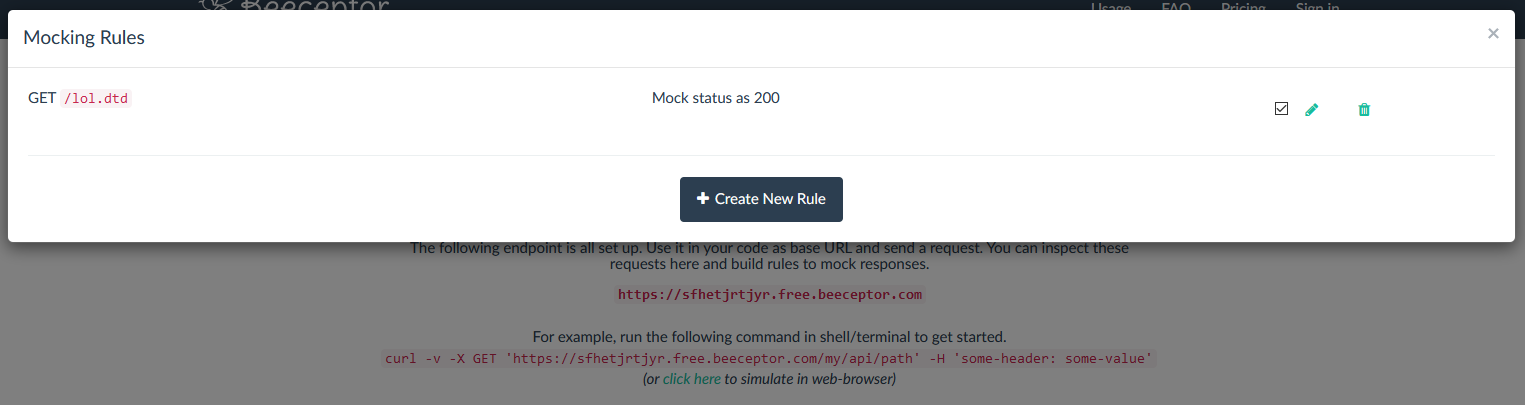
\includegraphics[scale=0.4]{images/Screenshot Beeceptor.png}

\begin{flushleft}
Impostiamo la regola in modo che la richiesta GET a lol.dtd serva il seguente contenuto:
\end{flushleft}

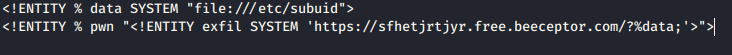
\includegraphics[scale=0.4]{images/Screenshot file lol.dtd.png}


\begin{flushleft}
Ora che abbiamo eseguito tutta la configurazione, tutto ciò che dobbiamo fare è reimpacchetare/comprimere il file MTGL e inviarlo alla vittima (nel nostro esperimento, siamo noi stessi ad impersonare la vittima e ad aprire il file payload.mtgl).
\end{flushleft}


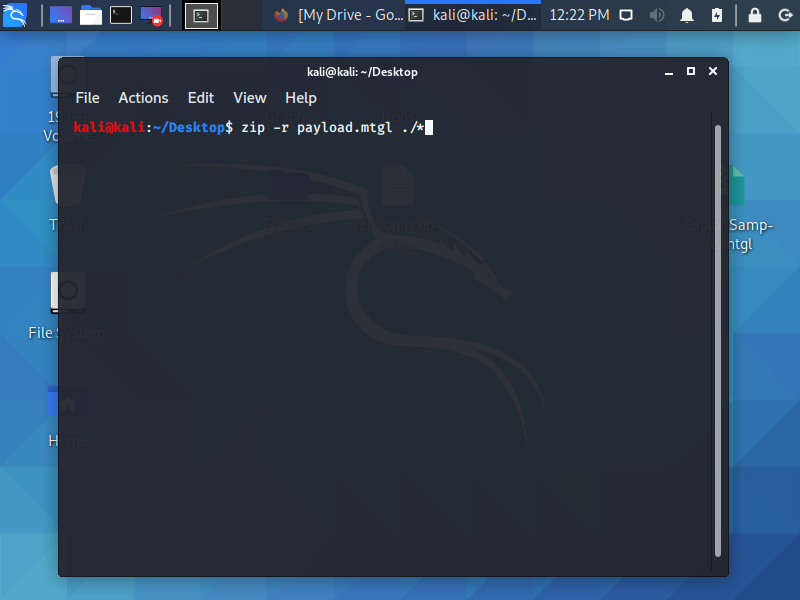
\includegraphics[scale=0.4]{images/Screenshot zip file MTGL.png}

\begin{flushleft}
Provando ad aprire il file payload.mtgl con Maltego, vedremo che su Beeceptor, in particolare su https://sfhetjrtjyr.free.beeceptor.com, comparirà il contenuto del file /etc/subuid. L'attacco ha dunque avuto l'effetto atteso.
\end{flushleft}


\chapter{Interpretazioni personali e conclusioni}
\begin{flushleft}
Dalla versione 4.2.12 non è più possibile sfruttare questa vulnerabilità. Questo mette in luce due aspetti:

\begin{itemize}
    \item è importante tenere sotto costante aggiornamento i propri sistemi software, spesso è possibile risolvere una vulnerabilità semplicemente scaricando l'ultima versione del prodotto software utilizzato.
    
    \item attraverso l'uso di tecniche di ingegneria sociale, l'attaccante potrebbe ingannare la vittima, facendole credere di essere un membro del team di progetto che vuole condividere un file MTGL/MTZ. Se la vittima si fida e accetta di scaricare e aprire il file, allora l'attacco ha successo. Questo mette in luce come un'attacco si basi sia su una componente tecnica (i tecnicismi dell'attacco), sia su una componente umana (le tecniche di ingegneria sociale adoperate). \'E fondamentale quindi riuscire a capire, nel limite del possibile, la vera identità del proprio interlocutore, ed educare il proprio team circa i rischi legati all'uso dell'ingegneria sociale e ai modi con cui ci si può difendere da quest'ultima.
    
\end{itemize}

\end{flushleft}

%\chapter{Conclusioni}
%\begin{itemize}
    \item Maltego: https://en.wikipedia.org/wiki/Maltego
    \item Vulnerabilità XXE: https://portswigger.net/web-security/xxe
    \item Descrizione vulnerabilità Maltego: https://www.hackersforchange.com/post/maltego-cve-2020-24656-analysis
    \item OSINT: https://www.recordedfuture.com/open-source-intelligence-definition/
    \item Maltego: https://docs.maltego.com/support/solutions/articles/15000019166-what-is-maltego-
\end{itemize}

\chapter{Bibliografia}
\begin{itemize}
    \item Maltego: https://en.wikipedia.org/wiki/Maltego
    \item Vulnerabilità XXE: https://portswigger.net/web-security/xxe
    \item Descrizione vulnerabilità Maltego: https://www.hackersforchange.com/post/maltego-cve-2020-24656-analysis
    \item OSINT: https://www.recordedfuture.com/open-source-intelligence-definition/
    \item Maltego: https://docs.maltego.com/support/solutions/articles/15000019166-what-is-maltego-
\end{itemize}


\end{document}
